\section{Introduction}

The most efficient cryptographic protocols are symmetric, in that they use a single shared key.
To securely exchange a shared key, public key cryptography is used. Public key cryptography
relies on a public key for encryption and a private key for decryption, as first described by
Diffie and Hellmann.

Elliptic Curve Cryptography (ECC) is based on the properties of elliptic curves.
An elliptic curve is a curve \(E\) that is symmetric around the x-axis (see Figure \ref{fig:graphs}),
and can be described with the formula:

\begin{equation} \label{eq:elliptic-curve-formula-full}
	E: y^2 + a_1xy + a_3y = x^3 + a_2x^2 + a_4x + a_6
\end{equation}

Any elliptic curve can have its formula reduced to a much simpler form, which -- unlike the original
form -- is used in cryptography (see Section \ref{sec:math_curve}):

\begin{equation}
	E: y^2 = x^3 + ax + b
\end{equation}

When using elliptic curves for cryptography, a large prime \(p\) is selected, and the curves are defined
over a prime field \(\mathbb{F}_p\) of integers.

\begin{figure}[htb]
	\centering
	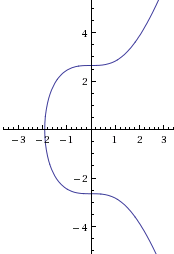
\includegraphics[width=0.37\textwidth]{introduction/secp256k1-graph}
	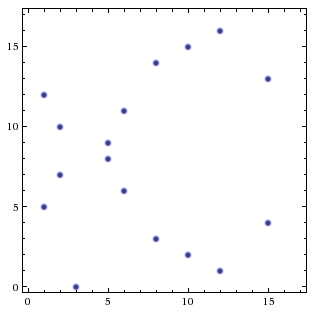
\includegraphics[width=0.52\textwidth]{introduction/secp256k1-graph-over-field-p17}
	\caption{The curve \(E: y^2 = x^3 + 0x + 7\) depicted left, and the same curve over the prime field
		\(\mathbb{F}_{17}\) depicted right.}
	\label{fig:graphs}
\end{figure}

Each curve, in addition to all the regular points, contains a point at infinity, \(O_\infty\). For example, a
curve \(E: y^2 = x^3 + 7\) over a prime field \(\mathbb{F}_{17}\) can be written as:

\begin{equation}
	E(\mathbb{F}_{17}) = \{ O_\infty; (1,5); (1,12); ...; (15,13) \}
\end{equation}

ECC relies on the hardness of the elliptic curve discrete logarithm problem (ECDLP) to be secure. ECDLP is
defined as such: ``given an elliptic curve \(E\) defined over a finite field \(\mathbb{F}_q\), a point
\(P \in E(\mathbb{F}_q)\) of order \(n\), and a point \(Q \in \langle P \rangle\), find the integer
\(l \in [0,n-1]\) such that \(Q = lP\). The integer \(l\) is called the \emph{discrete logarithm of
\(Q\) to the base \(P\)}, denoted \(l = log_P Q\).''\footnote{The hardness of the adapted ElGamal (see
Section \ref{sec:math_encryption}) is exactly that of the ECDLP, with the public key \(Q\) and private
key \(l\).}\cite{hankerson2010}

The order \(n\) of \(P\) is a number such that \(nP = O_{\infty}\) (the point at infinity), and is used to describe
the cyclic subgroup \(\langle G \rangle = \{ O_\infty, P, 2P, ..., (n-1)P \} \). For a generator, this cyclic subgroup
will contain all of the points on the curve.

There are several other concerns than the ECDLP to be considered when evaluating the safety of using a curve. Bernstein and Lange
provide an extensive list of requirements for the safety of curves, including indistinguishability from uniform random
strings, and ``simple, fast, constant-time, single-coordinate single-scalar multiplication''. They also list a variety
of curves, noting which of the requirements they fulfil.\cite{safecurves} Per Bernstein and Lange's definition none of
the curves described in detail in this report can be considered safe.

\subsection{In this report ---}

Elliptic curves provide a new mathematical model that can be used as the basis for cryptography. Several
implementations of ECC already exist: Bouncy Castle is a free Java and C\# implementation of various cryptosystems,
including some based on elliptic curves.\cite{bouncycastle}

In 1995, ElGamal described a simple (as in simply brilliant) public key cryptosystem that can be adapted
to use elliptic curves (Section \ref{sec:math_encryption_elgamal}). This system relies on the ability to
encode messages as points on an elliptic curve (Section \ref{sec:math_encoding}).

The implementation is modular, allowing for different curves and encryption schemes to be swapped in and out
rapidly (Section \ref{sec:implementation}). As such, the library can be extended in the future to support different
curves, encodings, and encryption schemes. It also provides a readable syntax that is closer to natural mathematical
syntax than available alternatives, such as Bouncy Castle (Section \ref{sec:implementation_curves}).

While \emph{OpenECC} implements the constructs used specifically in elliptic curve cryptography it relies one external construct.
The elliptic curves rely on Bouncy Castle library's implementation of finite fields.

This report describes the structure of \emph{OpenECC}, an open-source implementation of the functionality
described in the mathematical foundation section. \emph{OpenECC} has been developed concurrently with the
production of the report, and is used as a basis for performance measurements.

Several multiplication algorithms are compared with each other (Section \ref{sec:performance_multipliers});
the encryption of a string is broken down and the distribution of time spent in different parts of the program
is discussed (Section \ref{sec:performance_components}); and finally, OpenECC is compared to Bouncy Castle to
get an indication of the real-world applicability of the implementation (Section \ref{sec:performance_bouncycastle}).

OpenECC is by no means a complete library that should be used in production. It should not be used to encrypt real,
sensitive data (see Appendix \ref{app:disclaimer}).

The code for OpenECC can be found at \texttt{https://github.com/hypesystem/OpenECC}, and it is recommended to look
through it while to see concrete implementations of the algorithms and calculations described in Section
\ref{sec:math} and to see how the architecture described in Section \ref{sec:implementation} dictates the design
of the library.